\documentclass[fleqn]{article}

\usepackage{graphicx}
\usepackage{xurl}
\usepackage{url}
\usepackage{caption}
\usepackage{fancyhdr}
\usepackage{mathtools}
\usepackage{amsmath}
\usepackage{amssymb}
\usepackage{tikz}
\usepackage{listings}
\usepackage{xcolor}
\usepackage{float}

\definecolor{codegreen}{rgb}{0,0.6,0}
\definecolor{codegray}{rgb}{0.5,0.5,0.5}
\definecolor{codepurple}{rgb}{0.58,0,0.82}
\definecolor{backcolour}{rgb}{0.95,0.95,0.92}

\lstdefinestyle{mystyle}{
    backgroundcolor=\color{backcolour},   
    commentstyle=\color{codegreen},
    keywordstyle=\color{magenta},
    numberstyle=\tiny\color{codegray},
    stringstyle=\color{codepurple},
    basicstyle=\ttfamily\footnotesize,
    breakatwhitespace=false,         
    breaklines=true,                 
    captionpos=b,                    
    keepspaces=true,                 
    numbers=left,                    
    numbersep=5pt,                  
    showspaces=false,                
    showstringspaces=false,
    showtabs=false,                  
    tabsize=2
}

\lstset{style=mystyle}

\usepackage{xepersian}

\settextfont[BoldFont={XB Zar bold.ttf}]{XB Zar.ttf}
\setlength\parindent{0pt}



\newcommand{\expnumber}{چهارم}



\title{

\includegraphics[width=0.4\textwidth]{sharif.png}\\
\normalsize{دانشکده مهندسی کامپیوتر}\\
\vspace{1cm}
    
\huge{آزمایشگاه معماری کامپیوتر}
\\ \vspace{.8cm}
\Large{گزارش آزمایش \expnumber}
\\ \vspace{.8cm}
\Large{عنوان آزمایش : جمع/تفریق کننده ممیز شناور}
}

\author{
\\
دکتر حمید سربازی آزاد
\\ \vspace{.4cm}
\\
  سارا آذرنوش       ---      98170668
\\ \vspace{0.2cm} \\
  کسری امانی       ---      98101171
\\ \vspace{0.2cm} \\
  پارسا محمدیان       ---      98102284
\\ \vspace{.4cm}
}

\date{\today}

\begin{document}

\clearpage\maketitle
\thispagestyle{empty}

\newpage

\pagestyle{fancy}
\lhead{آزمایشگاه معماری کامپیوتر}

\rhead{آزمایش \expnumber}

\tableofcontents

\setcounter{page}{1}

\newpage

\section{مقدمه}
\lr{Binary Coded Decimal} 
یا 
\lr{BCD} 
یک نحوه کد گذاری اعداد دهدهی با استفاده از بیت‌ها و ارقام باینری است. در این روش 
کد گذاری، هر رقم دهدهی را با 4 بیت یا رقم باینری مشخص می‌کنند. این روش کد گذاری 
در برخی زمینه‌ها برتری دارد و مورد استفاده است. با این حال برخی مواقع نیاز داریم 
برای انجام محاسبات اعداد 
\lr{BCD} 
را به باینری تبدیل کنیم. در این آزمایش نیز میخواهیم یک مبدل 
\lr{BCD}
به 
\lr{Binary}
طراحی و پیاده‌سازی کنیم.

\section{هدف آزمایش}
در این آزمایش یک مبدل عدد دهدهی سه رقمی (که با 12 بیت نمایش داده می‌شود) 
به عدد دودویی ده بیتی (چون بزرگترین عدد یعنی 999 ده بیت نیاز دارد) 
می‌سازیم. این مبدل یک مدار ترتیبی است لذا برای شروع و پایان عملیات از سیگنال‌های 
\lr{Start}
و
\lr{End}
استفاده می‌کنیم.

\section{شرح آزمایش}
ابتدا نمودار 
\lr{ASM}
مبدل خواسته شده را با توجه به مراحل ذکر شده در دستورکار رسم می‌کنیم. این 
نمودار 
\lr{ASM}
دارای سه بلوک است که تصویر آن در شکل 
\ref{asm}
آمده است.

\begin{figure}[!htbp]
    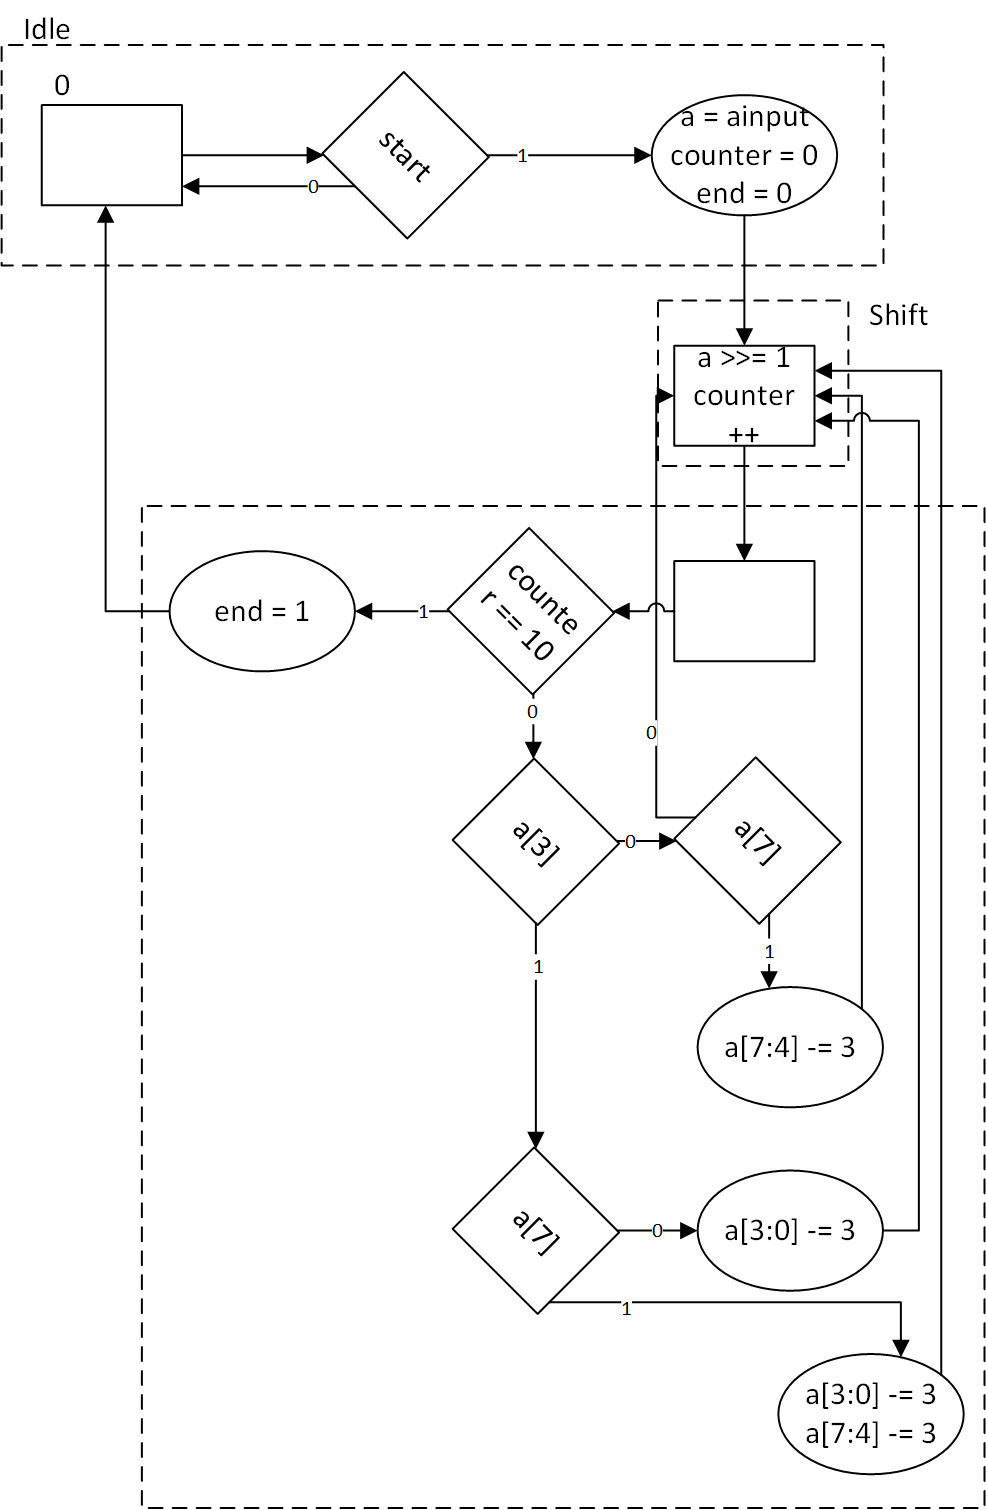
\includegraphics[width=\textwidth]{Assets/ASM.png}
    \caption{نمودار \lr{ASM}}
    \label{asm}
\end{figure}

سپس با توجه به نمودار 
\lr{ASM}
نمودار حالت مدار مطلوب را بدست می‌آوریم. تصویر نمودار حالت در شکل 
\ref{sd}
آمده است. 

\begin{figure}[!htbp]
    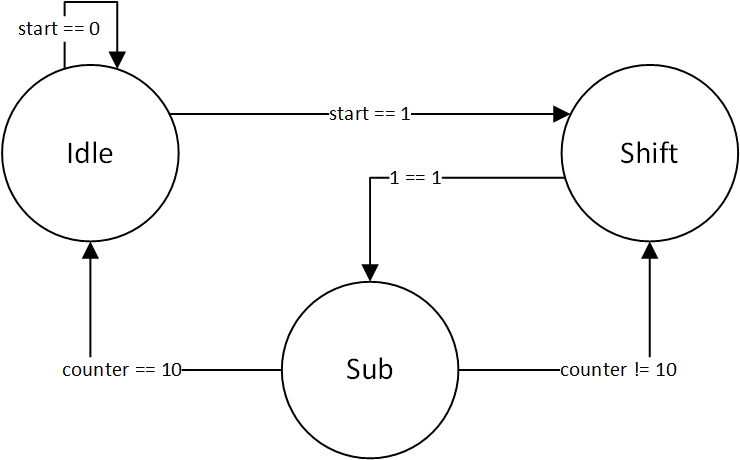
\includegraphics[width=\textwidth]{Assets/SD.png}
    \caption{نمودار حالت}
    \label{sd}
\end{figure}

حال به سراغ پیاده سازی می‌رویم و با نمودار حالت بدست آمده واحد کنترل مدار را 
طراحی می‌کنیم. در این واحد کنترل به ازای هر حالت از یک فلیپ فلاپ نوع دی استفاده 
شده است.

سپس به سراغ مسیر داده می‌رویم و با جایگذاری قطعات مناسب آن را طراحی می‌کنیم. سپس 
سیگنال‌های کنترلی را متصل می‌کنیم. تصویر مدار نهایی در شکل 
\ref{circ}
آمده است.

\begin{figure}[!htbp]
    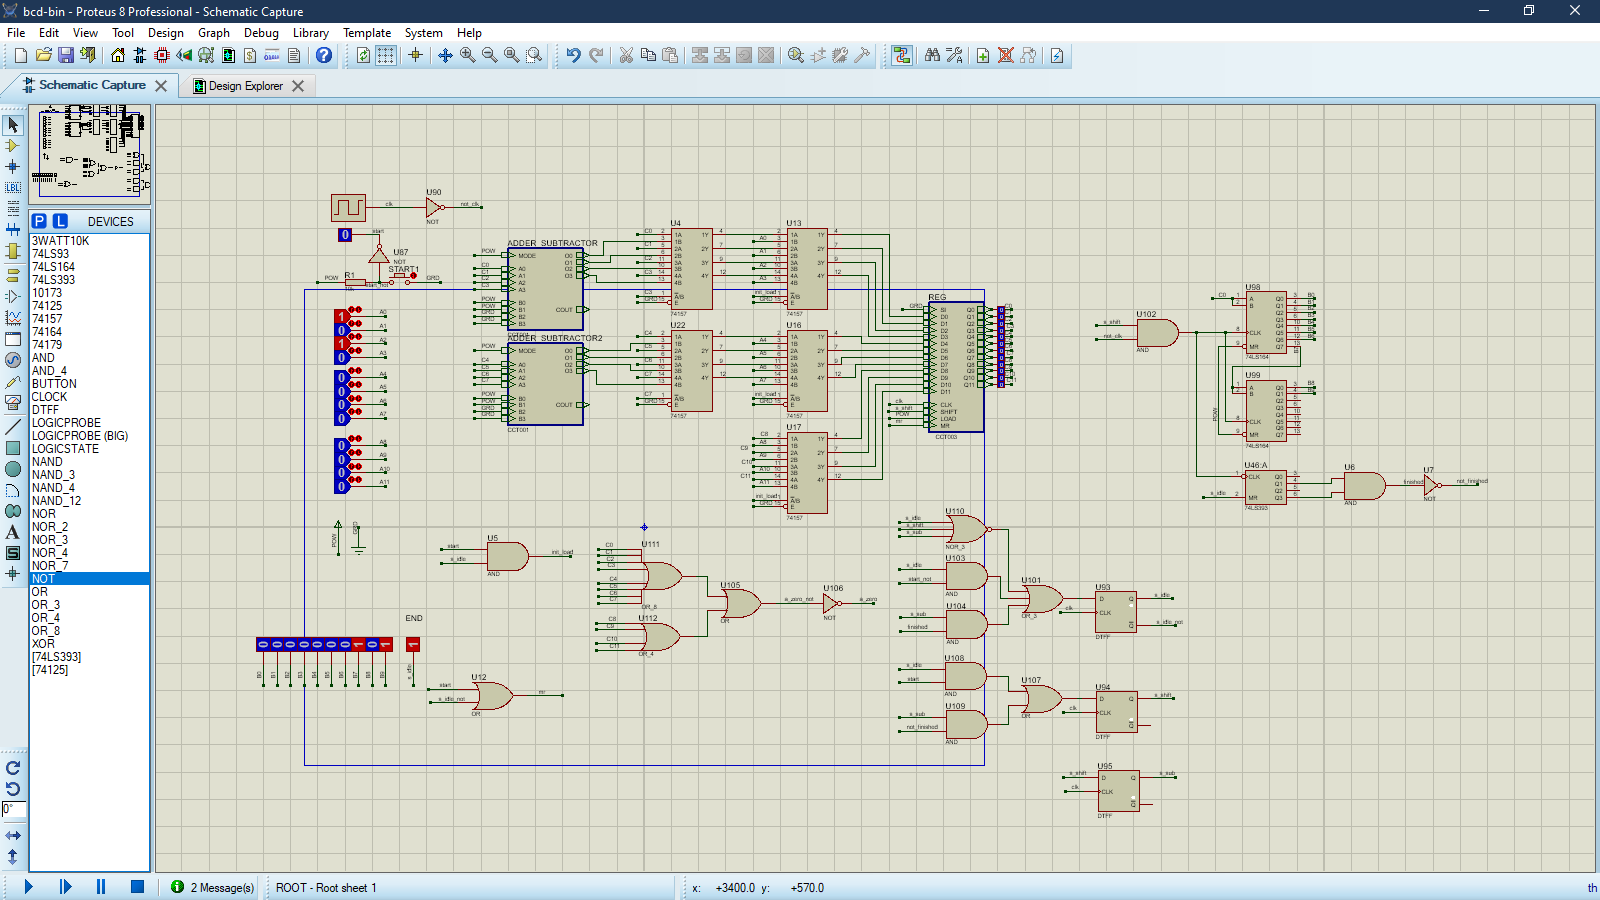
\includegraphics[width=\textwidth]{Assets/circuit.png}
    \caption{مدار نهایی}
    \label{circ}
\end{figure}

\section{نتیجه آزمایش}
در آخر یک مدار مبدل دهدهی سه رقمی به دودویی داریم که با دادن عدد ورودی و فشردن 
دکمه استارت شروع به کار می‌کند. در آخر پس از گذشت کلاک متناسب، عدد دودویی را در خروجی نمایش 
می‌دهد. 

برای تست مدار چند ورودی متفاوت را بررسی می‌کنیم که در اشکال 
\ref{t1}
\ref{t2}
\ref{t3}
\ref{t4}
\ref{t5}
قابل مشاهده هستند.

\begin{figure}[!htbp]
    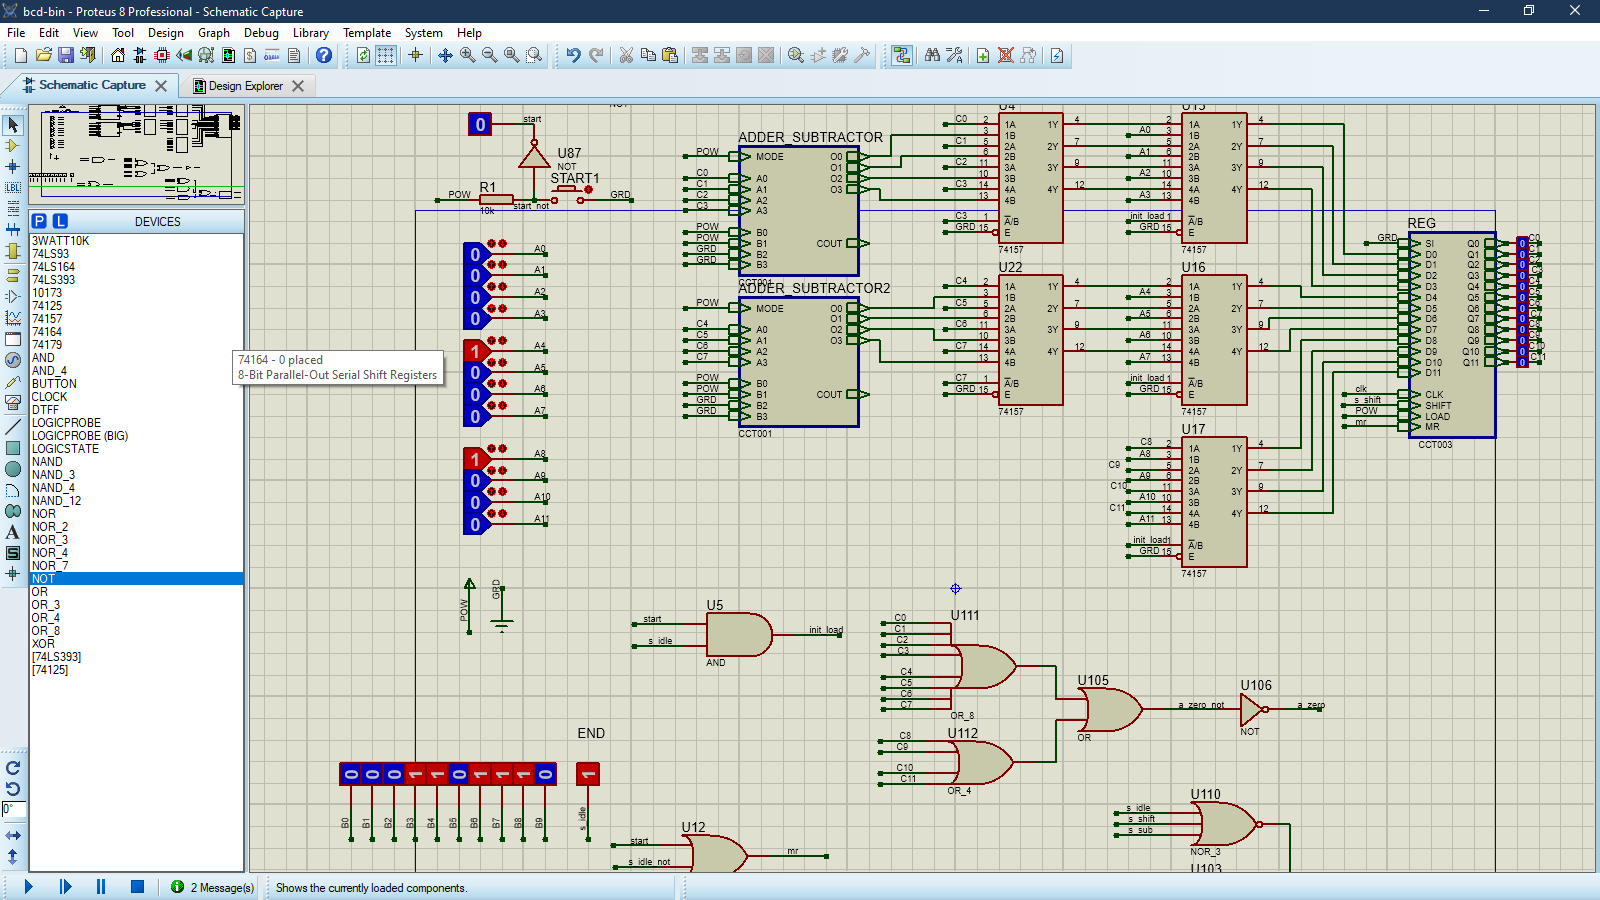
\includegraphics[width=\textwidth]{Assets/t1.png}
    \caption{تست 1 - عدد 110}
    \label{t1}
\end{figure}

\begin{figure}[!htbp]
    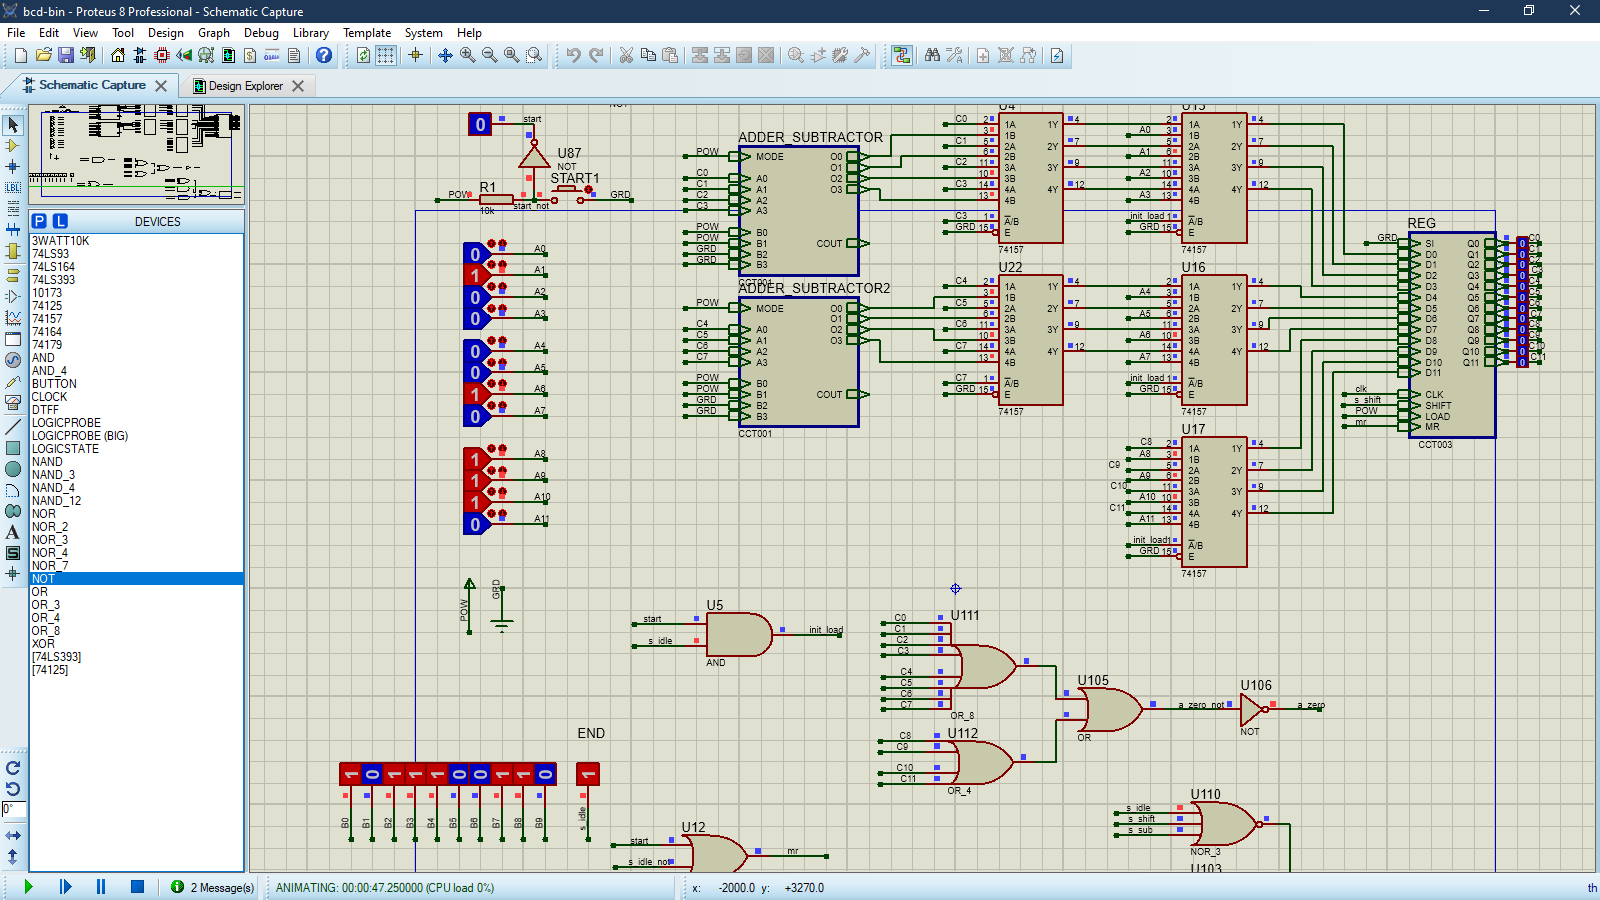
\includegraphics[width=\textwidth]{Assets/t2.png}
    \caption{تست 2 - عدد 742}
    \label{t2}
\end{figure}

\begin{figure}[!htbp]
    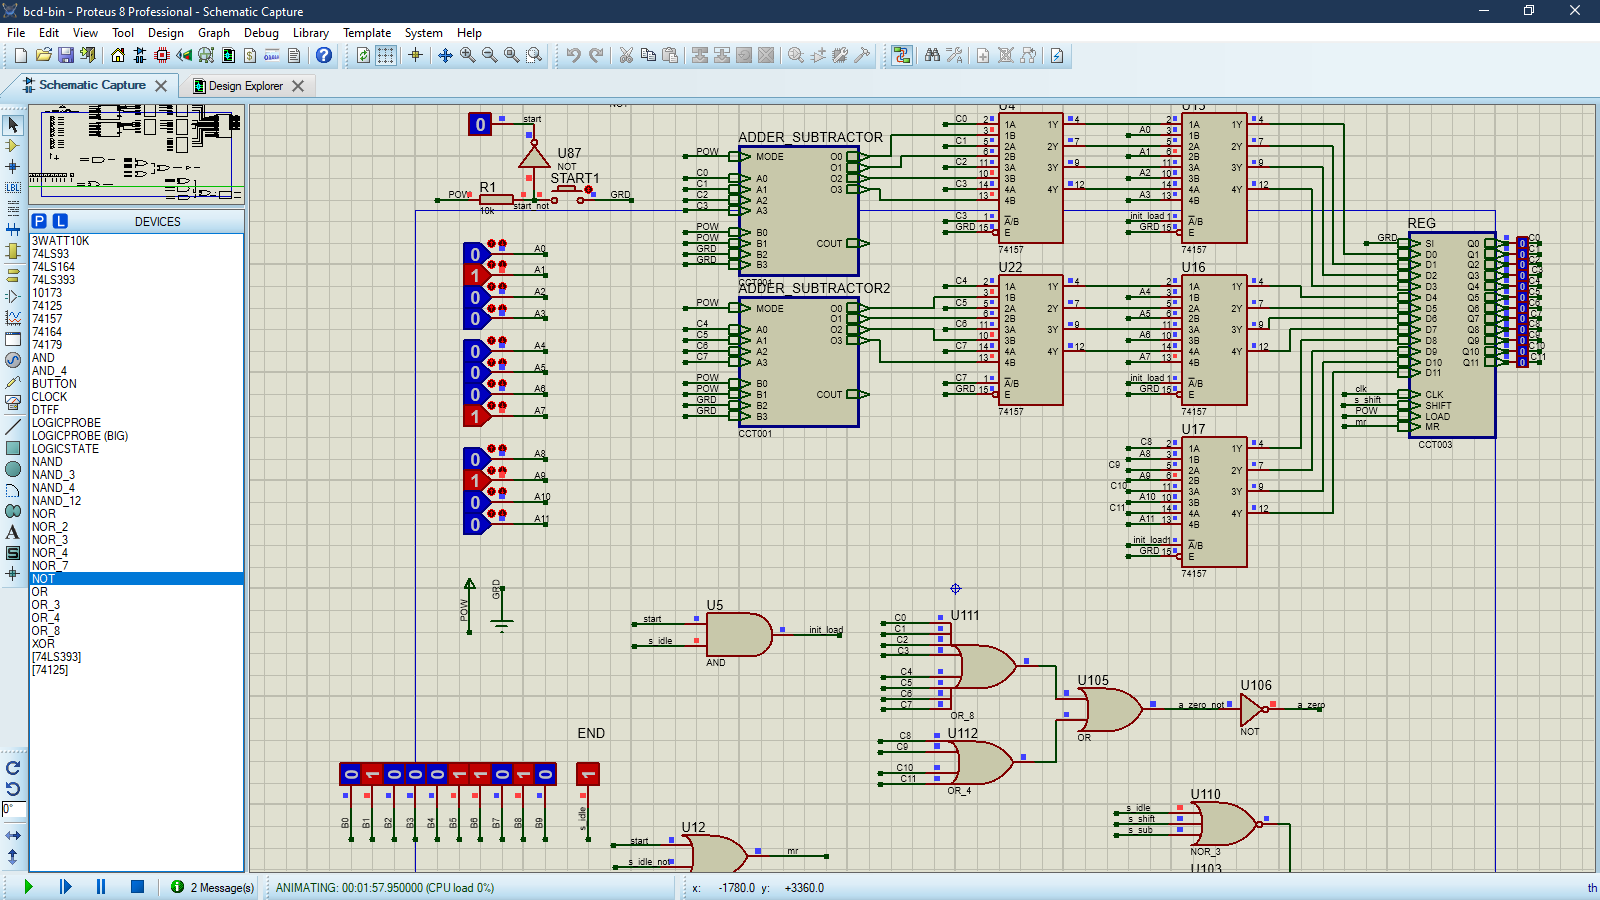
\includegraphics[width=\textwidth]{Assets/t3.png}
    \caption{تست 3 - عدد 282}
    \label{t3}
\end{figure}

\begin{figure}[!htbp]
    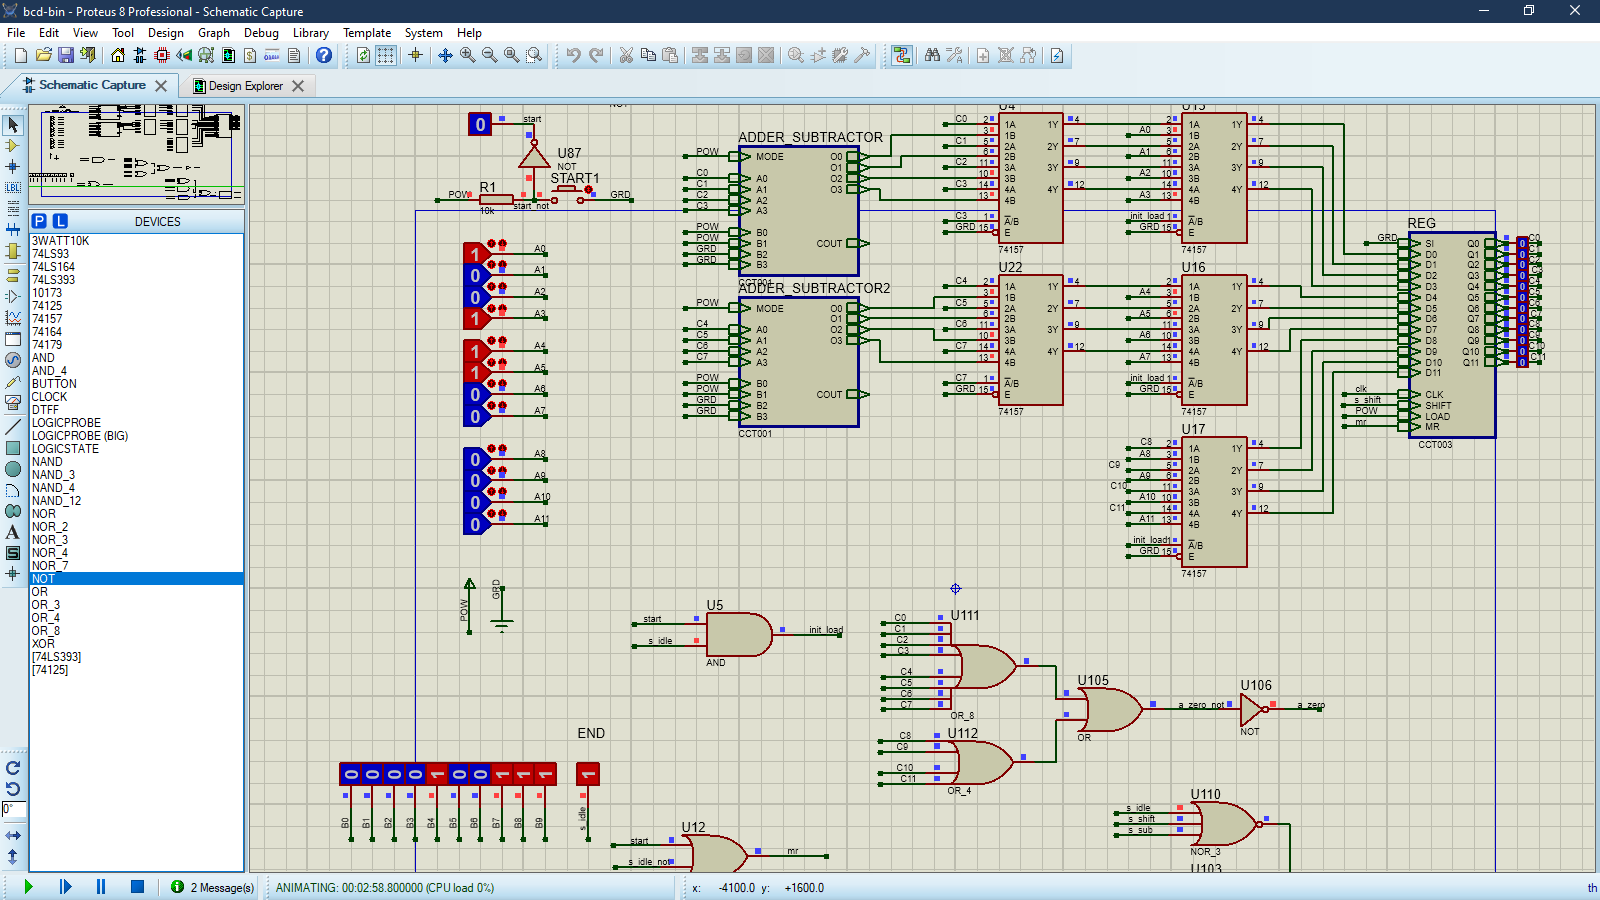
\includegraphics[width=\textwidth]{Assets/t4.png}
    \caption{تست 4 - عدد 39}
    \label{t4}
\end{figure}

\begin{figure}[!htbp]
    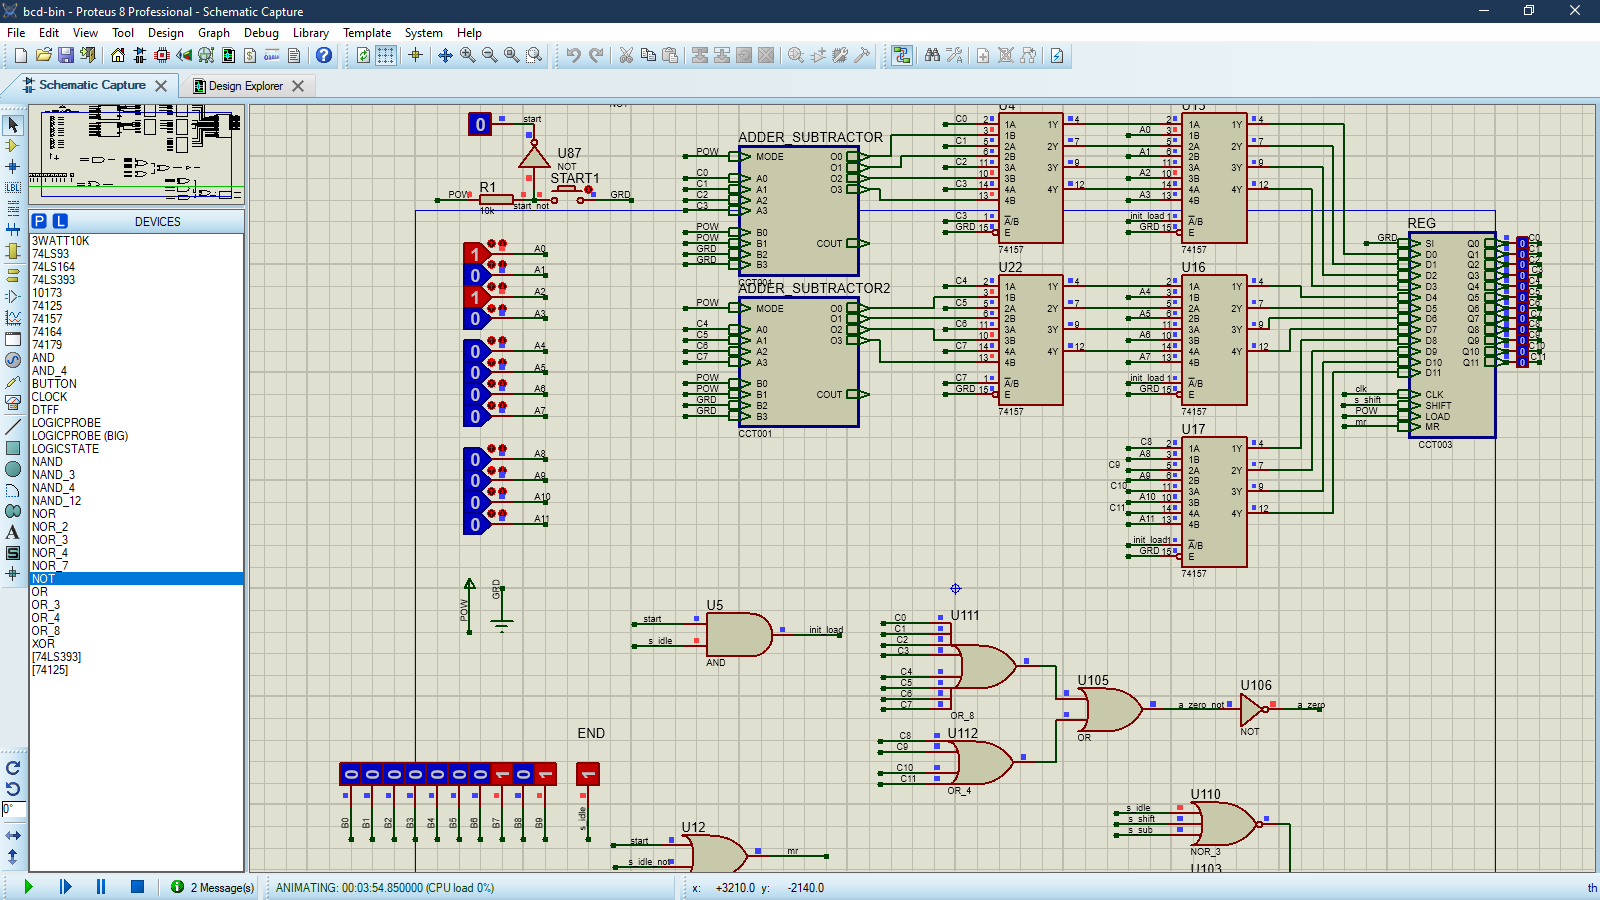
\includegraphics[width=\textwidth]{Assets/t5.png}
    \caption{تست 5 - عدد 5}
    \label{t5}
\end{figure}

\end{document}